% DAFN24 - Robotics - Lecture 7
% Roberto Masocco <roberto.masocco@uniroma2.it>
% June 4, 2024

\documentclass[aspectratio=169]{beamer}

% Slides layout
\usepackage[
    title={Inside the roboticist’s toolbox},
    subtitle={Linux kernel, Docker, and more},
    event={DAFN},
    author={Roberto Masocco},
    longauthor={Roberto Masocco},
    email={roberto.masocco@uniroma2.it},
    institute={Tor Vergata},
    longinstitute={University of Rome Tor Vergata},
    department={Department of Civil Engineering and Computer Science Engineering},
    researchgroup={},
    date={June 5, 2024}
]{utvengbeamer}

% Code listings settings
\usepackage[nomath]{lmodern}
\definecolor{codegreen}{rgb}{0 0.5 0}
\definecolor{codered}{rgb}{1 0 0}
\definecolor{codeocher}{rgb}{0.8 0.47 0.13}
\usepackage{listings}
\lstdefinestyle{beamer}{
    basicstyle=\ttfamily\small,
    commentstyle=\color{codegreen},
    breakatwhitespace=false,
    captionpos=b,
    frame=lines,
    keepspaces=true,
    keywordstyle=\color{codered}\bfseries,
    numbers=left,
    numbersep=5pt,
    numberstyle=\footnotesize,
    showspaces=false,
    showstringspaces=false,
    showtabs=false,
    stringstyle=\color{codeocher},
    tabsize=2
}
\lstset{style=beamer}
\lstdefinelanguage{Dockerfile}{
  alsoletter={[, ], _, /},
  morecomment=[l][\color{codegreen}]{\#},
  morekeywords={FROM, RUN, ADD, COPY, LABEL, ENV, ARG, CMD}
}
\lstdefinelanguage{compose}{
  alsoletter={:, -, /},
  morecomment=[l][\color{codegreen}]{\#},
  morekeywords={services:, build:, context:, network_mode:, args:, environment:, command:, volumes:, image:, -}
}

\usepackage{hyperref}
\usepackage{wasysym}

\begin{document}

% --- Title page ---
\frame{\titlepage}

% --- Table of contents ---
\begin{frame}
\frametitle{Roadmap}
\tableofcontents
\end{frame}

% --- Section 1 ---
% Section 1 - Containers
% Roberto Masocco <roberto.masocco@uniroma2.it>
% June 4, 2024

% ### Containers ###
\section{Containers}
\graphicspath{{figs/section1/}}

% --- Why containers? ---
\begin{frame}{Why containers?}
	\begin{exampleblock}{Example: Packaging applications}
		Suppose you are ready to distribute your new application:
		\begin{itemize}
			\item you need to be sure that it is compatible with all the \textbf{platforms} you chose to support;
			\item you need to figure out a way to deal with \textbf{dependencies};
			\item you want to publish some kind of \textbf{self-contained}, easily-identifiable \textbf{package}.
		\end{itemize}
	\end{exampleblock}
\end{frame}
\begin{frame}{Why containers?}
	\begin{exampleblock}{Example: Isolating applications}
		Suppose you are deploying applications on a server:
		\begin{itemize}
			\item you want to define \textbf{resource quotas} and \textbf{permissions} for each;
			\item you want to be sure that each module has what it needs to operate, but \textbf{nothing more};
			\item you want to \textbf{isolate} each module for security reasons, in case something goes wrong.
		\end{itemize}
	\end{exampleblock}
\end{frame}
\begin{frame}{Why containers?}
	\begin{exampleblock}{Example: Replicating environments}
		Suppose you are developing applications for a specific system (maybe with a different architecture):
		\begin{itemize}
			\item you want to have a \textbf{software copy} of such system without having to carry it with you;
			\item you want to have all \textbf{libraries} and \textbf{dependencies} installed without tainting your own;
			\item you would like to \textbf{deploy} the entire installation with just a few commands.
		\end{itemize}
	\end{exampleblock}
\end{frame}
\begin{frame}{Why containers?}
	\begin{columns}
		\column{.5\textwidth}
		A possible solution to many of the previous situations could be a set of \textbg{virtual machines}.\\
		However, virtual machines are \textbg{slow}, hypervisors take up \textbg{system resources} and guest kernels must always be \textbg{tweaked}.
		\newline\newline
		In each of the above scenarios something simpler would be enough, especially since \textbg{the OS is not involved}, only applications are.
		\begin{block}{}
			\centering
			This is what a \textbf{container} is.
		\end{block}

		\column{.5\textwidth}
		\begin{figure}
			\centering
			
\includegraphics[scale=.7]{freebsdjail.png}
			\label{fig:jail}
			\caption{FreeBSD jail logo.}
		\end{figure}
	\end{columns}
\end{frame}

% --- Containers in the Linux kernel ---
\begin{frame}{Containers in the Linux kernel}
	\begin{columns}
		\column{.5\textwidth}
		Support for containers was added to the Linux kernel with a set of \textbg{features} starting from kernel 2.6 (2003), mainly:
		\begin{itemize}
			\item \textbg{control groups} (\texttt{cgroups}): defining different resource usage policies for groups of processes;
			\item \textbg{namespaces}: isolating processes and users in different "realms", both hardware (e.g. network stack) and software (e.g. PIDs);
			\item \textbg{capabilities}: granting some of the superuser's permissions to unprivileged threads.
		\end{itemize}

		\column{.5\textwidth}
		\begin{figure}
			\centering
			
\includegraphics[scale=.2]{tux.png}
			\label{fig:tux}
			\caption{Tux.}
		\end{figure}
	\end{columns}
\end{frame}
\begin{frame}{Containers in the Linux kernel}
	\begin{figure}
		\centering
		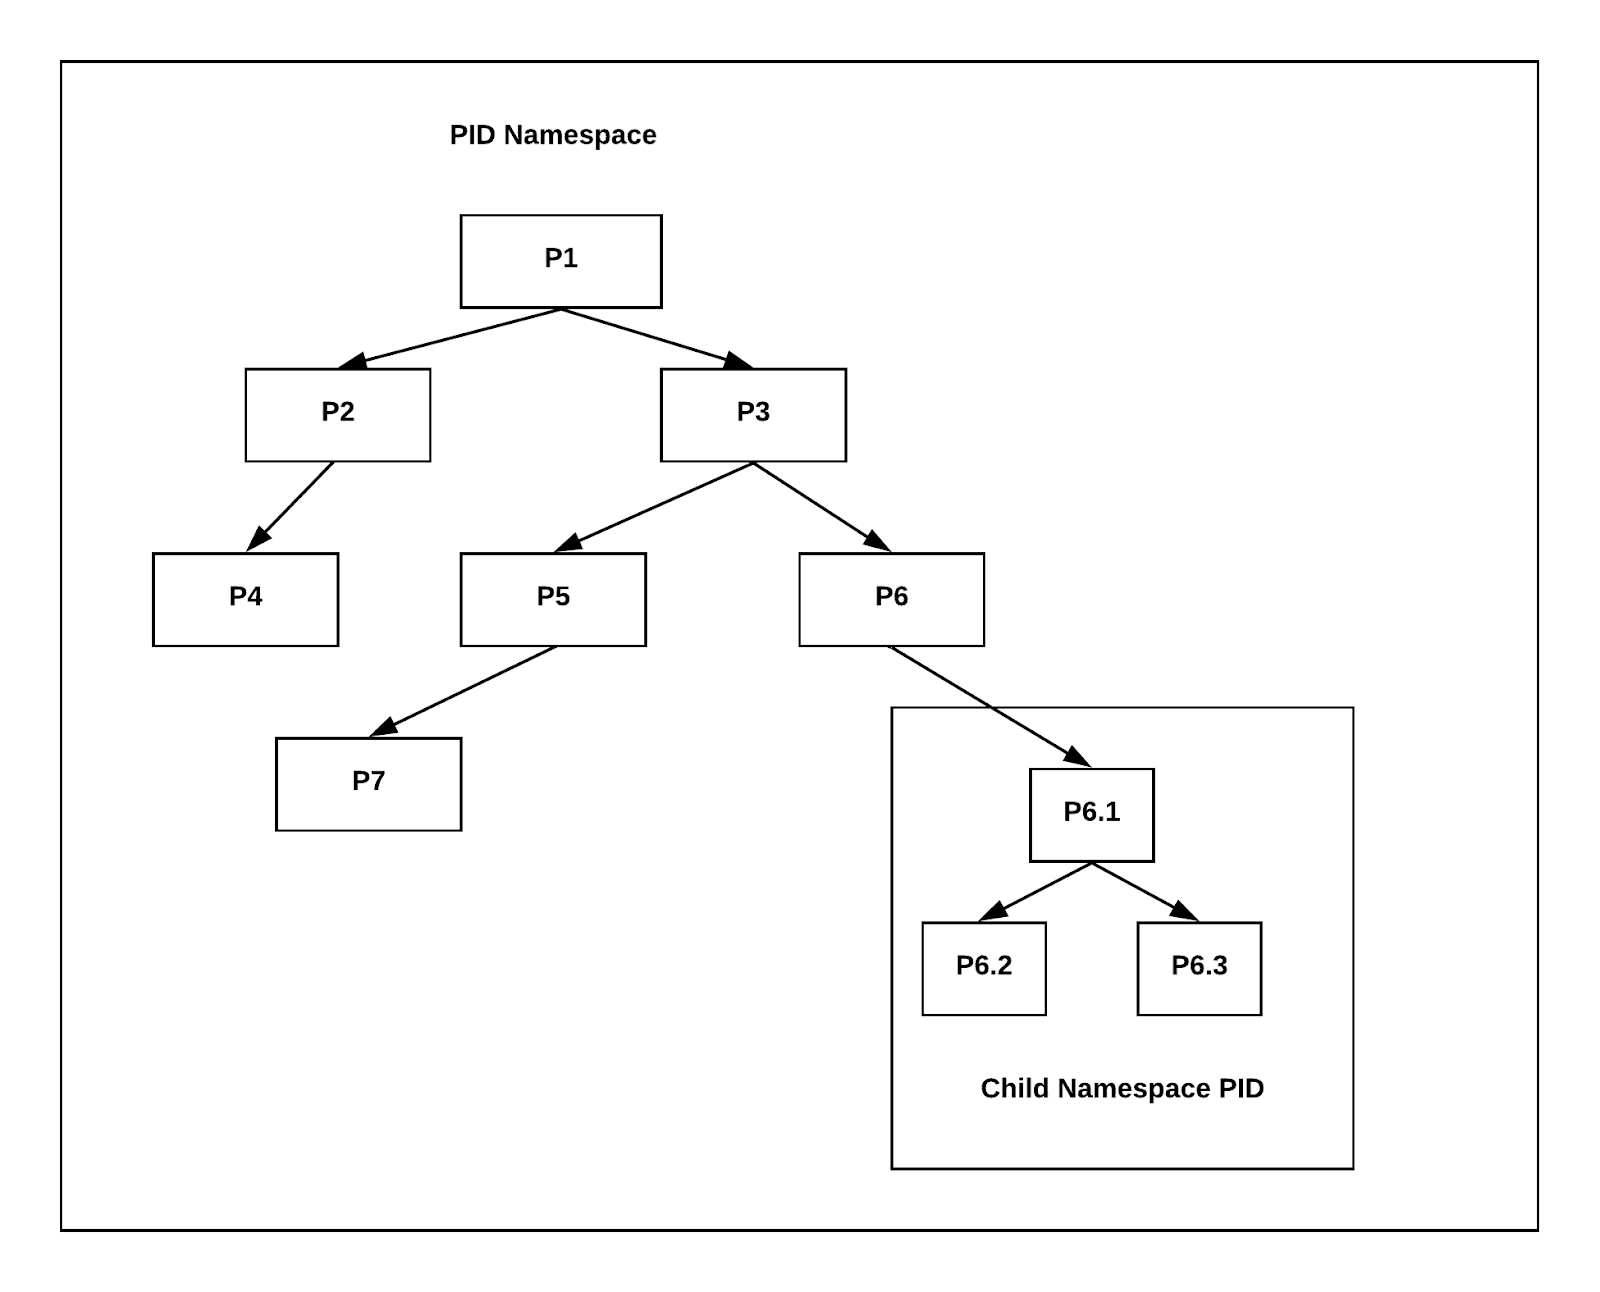
\includegraphics[scale=.137]{pidNamespace.png}
		\label{fig:pidnamespace}
		\caption{Nested PID namespaces.}
	\end{figure}
\end{frame}


% --- Section 2 ---
% Section 2 - Docker
% Roberto Masocco <roberto.masocco@uniroma2.it>
% June 4, 2024

% ### Docker ###
\section{Docker}
\graphicspath{{figs/section2/}}

% --- Docker Engine ---
\begin{frame}{Docker Engine}
	\begin{columns}
		\column{.5\textwidth}
		\textbg{Docker} is the currently de-facto standard for building, managing and distributing \textbg{multiplatform} containers.
		\newline\newline
		It is an engine (\emph{i.e.}, a collection of \textbg{daemons}) that automates the management of the kernel subsystems in order to set up, store and run containers.

		\column{.5\textwidth}
		\begin{figure}
			\centering
			\label{fig:docker}
			
\includegraphics[scale=.2]{docker.png}
			\caption{Docker logo.}
		\end{figure}
	\end{columns}
\end{frame}
\begin{frame}{Docker Engine}
	\begin{figure}
		\centering
		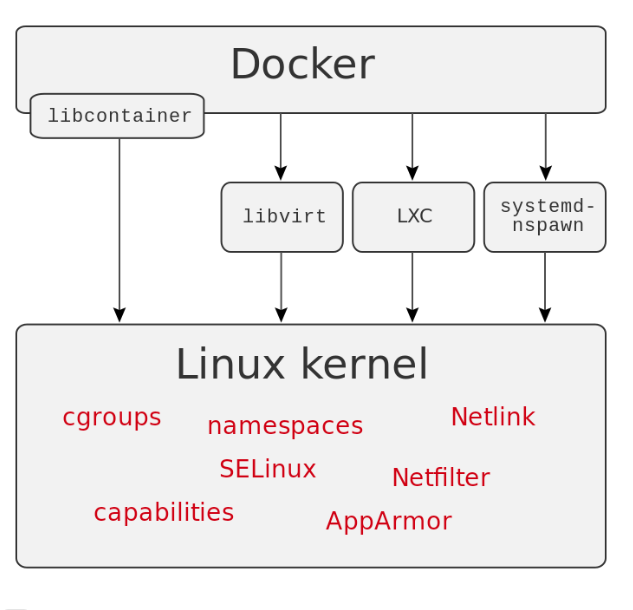
\includegraphics[scale=.29]{dockerScheme.png}
		\label{fig:dockerscheme}
		\caption{Docker Engine scheme.}
	\end{figure}
\end{frame}

% --- Containers in robotics ---
\begin{frame}{Containers in robotics}
	Containers can be of help in some classic scenarios:
	\begin{itemize}
		\item \textbg{deploying} applications or whole control architectures, solving issues like \textbg{dependencies} and \textbg{configurations};
		\item configuring and distributing \textbg{development environments};
		\item working with \textbg{multiple architectures} at the same time: Docker fully supports \href{https://www.qemu.org/}{\color{blue}\textbf{\underline{QEMU}}} to build and run containers;
		\item expanding the capabilities of \textbg{(partially) closed-source} hardware solutions (\emph{e.g.}, Nvidia Jetson...).
	\end{itemize}
\end{frame}

% --- Building a Docker container ---
\begin{frame}{Building a Docker container}{Step by step}
	\begin{enumerate}
		\item A \textbg{Dockerfile} specifies a set of rules to build an \textbg{image}, just like a script.
		\item \textbg{Images} are the binary archives from which a \textbg{container} can be started: they can be stored, pulled from a remote \textbg{registry} or simply built locally.
		\item A \textbg{container} can be built from an image and then started, stopped and managed by the Docker daemon.
		\item Processes started inside the container are subject to its limitations, \emph{e.g.}, \textbg{filesystem jails} prevent them to climb up to the hosts's filesystem.
	\end{enumerate}
	Images are built \textbg{incrementally}: each Dockerfile directive defines a new \textbg{layer}, and the Docker engine stores the differences between each build step thanks to \textbg{OverlayFS}.\\
	For every new container, its filesystem will be in a \textbg{new top layer}.\\
	This allows to efficiently \textbg{cache and share build stages}, which will then be stacked together to form images, but operating in a \textbg{copy-on-write}, \textbg{slower} fashion.
\end{frame}

% --- Dockerfiles ---
\begin{frame}[fragile]{Dockerfiles}
	\begin{columns}\column{.9\textwidth}
		\begin{lstlisting}[language=Dockerfile, caption=Minimal example of a Dockerfile running an Ubuntu image in a container.]
ARG VERSION=22.04
FROM ubuntu:$VERSION # Note the tag!

ENV DEBIAN_FRONTEND=noninteractive

RUN apt-get update && \
    apt-get install -y --no-install-recommends \
    build-essential \
    git && \
    rm -rf /var/lib/apt/lists/* /tmp/* /var/tmp/*/apt/lists/*

ENV DEBIAN_FRONTEND=dialog
LABEL maintainer.name="Roberto Masocco"
CMD ["bash"]
\end{lstlisting}
	\end{columns}
\end{frame}

% --- Dockerfile commands ---
\begin{frame}{Dockerfile commands}
	\begin{itemize}
		\item \texttt{FROM repository/image:tag}\\Specifies a base image to pull.
		\item \texttt{RUN command}\\Runs the following command in a new shell inside the container.
		\item \texttt{COPY source target}\\Copies a file into the container.
		\item \texttt{ENV variable=value}\\Sets an environment variable inside the container.
		\item \texttt{ARG name=value}\\Declares a build argument.
		\item \texttt{CMD ["command", "arg1", ...]}\\Specifies the command to run when the container is started.
	\end{itemize}
\end{frame}

% --- Docker commands ---
\begin{frame}{Docker commands}
	Again, just a few (each with a gazillion of options):
	\begin{itemize}
		\item \texttt{docker build}\\Builds a new image from a Dockerfile.
		\item \texttt{docker run}\\Builds and starts a container, optionally overriding the command (\texttt{CMD}).
		\item \texttt{docker ps}\\Lists active containers.
		\item \texttt{docker exec}\\Runs a command inside a container (\emph{e.g.}, a shell).
		\item \texttt{docker start}\\Starts a container.
	\end{itemize}
\end{frame}
\begin{frame}{Docker commands}
	\begin{itemize}
		\item \texttt{docker stop}\\Stops a container.
		\item \texttt{docker images}\\Lists available images.
		\item \texttt{docker rm}\\Removes a container.
		\item \texttt{docker rmi}\\Removes an image.
	\end{itemize}
	Containers and images are usually referenced by their \textbg{ID} (\emph{e.g.}, \texttt{abae6cae4648}).
	\newline\newline
	See the \href{https://docs.docker.com/engine/reference/builder/}{\color{blue}\underline{Dockerfile reference}} and the \href{https://docs.docker.com/engine/reference/commandline/docker/}{\color{blue}\underline{Docker CLI reference}} for more.
\end{frame}

% --- Containers on real robots ---
\begin{frame}{Containers on real robots}{Best practices}
  To run containers on embedded systems and robot SBCs, some configurations are suggested which \textbg{would not apply} in traditional containerization scenarios:
  \begin{itemize}
    \item the host \textbg{network stack} should be fully exposed to allow for \textbg{ROS} and other network-based \textbg{middleware} to work properly (\texttt{-{}-network host});
    \item the \textbg{IPC namespace} should be shared to allow for \textbg{shared memory} and \textbg{IPC} to work properly (\texttt{-{}-ipc host});
    \item to allow access to the \textbg{hardware} mounted on the host, one should grant full privileges to the container (\texttt{-{}-privileged}) and mount \texttt{/dev} and \texttt{/sys} inside it (\texttt{-v /dev:/dev -v /sys:/sys});
    \item your development directory should be \textbg{mounted as a volume} inside the container, so that file manipulations happen on the host filesystem (\texttt{-v /your/code:/workspace}).
  \end{itemize}
  We would like some utility to \textbg{automate} this process...
\end{frame}


% --- Section 3 ---
% Section 3 - Docker Compose
% Roberto Masocco <roberto.masocco@uniroma2.it>
% June 4, 2024

% ### Docker Compose ###
\section{Docker Compose}
\graphicspath{{figs/section3/}}

% --- Composing services ---
\begin{frame}{Composing services}
	\begin{columns}
		\column{.5\textwidth}
		Managing multiple, interdependent \textbg{containerized services} can become quite a tedious task.
    \newline\newline
		Each container may take multiple options, some have to be started in sequence or built in a particular way...
		\begin{block}{}
			\centering
			\textbf{Compose} is a utility that helps to \textbf{build}, \textbf{run} and \textbf{manage} multiplatform containers by parsing all such settings from \textbf{YAML configuration files}.
		\end{block}
    For instance, \textbg{our code repository} cointains development containers managed by Compose.

		\column{.5\textwidth}
		\begin{figure}
			\centering
			
\includegraphics[scale=.25]{composeLogo.png}
			\label{fig:compose}
			\caption{Docker Compose logo.}
		\end{figure}
	\end{columns}
\end{frame}

% --- Compose files ---
\begin{frame}[fragile]{Compose files}
	\begin{columns}\column{.9\textwidth}
		\begin{lstlisting}[language=compose, caption=Minimal example of a Compose file.]
services:
  development:
    build:
      context: .
      args:
        TARGET: dev
    image: devenv:latest
    environment:
      TERM: xterm-256color
    network_mode: host
    command: ["/bin/zsh"]
    volumes:
      - ~/.ssh:/home/user/.ssh
\end{lstlisting}
	\end{columns}
	Refer to the \href{https://docs.docker.com/compose/compose-file/}{\color{blue}\underline{Compose reference}} for more.
\end{frame}

% --- Compose commands ---
\begin{frame}{Compose commands}
	Pretty much the same that Docker has, but invoked with
  \newline\newline
	\texttt{docker-compose}
  \newline\newline
	instead of \texttt{docker}, and oriented only towards services specified in the local Compose file.
  \newline\newline
	See the \href{https://docs.docker.com/compose/reference/}{\color{blue}\underline{Compose CLI reference}} for more.
  \newline\newline
  Installation instructions for Docker and Compose can be found \href{https://docs.docker.com/engine/install/ubuntu/}{\color{blue}\underline{here}} and \href{https://docs.docker.com/compose/install/linux/}{\color{blue}\underline{here}}, respectively, and also in the provided shell script \href{https://github.com/IntelligentSystemsLabUTV/ros2-examples/blob/humble/bin/docker_install.sh}{\color{blue}\underline{\texttt{bin/docker\_install.sh}}}.\\
  On systems with an Nvidia GPU, the \href{https://docs.nvidia.com/datacenter/cloud-native/container-toolkit/overview.html}{\color{blue}\underline{NVIDIA Container Toolkit}} is suggested.\\
  Installation on Windows and macOS requires \href{https://www.docker.com/products/docker-desktop/}{\color{blue}\underline{Docker Desktop}}.
\end{frame}


\end{document}
